\documentclass[a4paper]{article}
\usepackage[utf8]{inputenc}
\usepackage[a4paper, left=2.5cm, right=2.5cm, top=2cm, bottom=2cm]{geometry}
\usepackage{lmodern}
\usepackage[T1]{fontenc}
\usepackage{graphicx}
\usepackage{amssymb}
\usepackage[utf8]{inputenc}
\usepackage{pgfplots}
\pgfplotsset{width=8cm,compat=1.9}
\usepackage{multicol}
\usepackage{csquotes}
\usepackage{amsfonts}
\usetikzlibrary{angles, quotes}

\newcommand{\overbar}[1]{\mkern 1.5mu\overline{\mkern-1.5mu#1\mkern-1.5mu}\mkern 1.5mu}
\renewcommand{\thesection}{\Alph{section}}
\renewcommand{\thesubsection}{\arabic{subsection}}
\renewcommand{\thesubsubsection}{(\emph{\alph{subsubsection}})}

\title{Ondes et particules}
\author{Hugo Lageneste}
\date{Février 2020}

\begin{document}

{Hugo \textsc{Lageneste}}\\
{Physique-Chimie - Ondes et particules}

\begin{center}
 \newcommand{\HRule}{\rule{\linewidth}{0.5mm}}
 {\huge \bfseries Ondes et particules}\\[0.1cm]
\end{center}

\section{Caractérisation des ondes}
\subsection{Direction de la perturbation}
{Une onde se propage longitudinalement lorsque la perturbation se fait parallèlement à la direction de propagation}\\
{Une onde se propage transversalement lorsque la perturbation se fait perpendiculairement à la direction de propagation}

\subsection{Période et fréquence}
{La période $T$ est la durée pour qu'un point revienne dans un même état vibratoire}
\begin{center}
	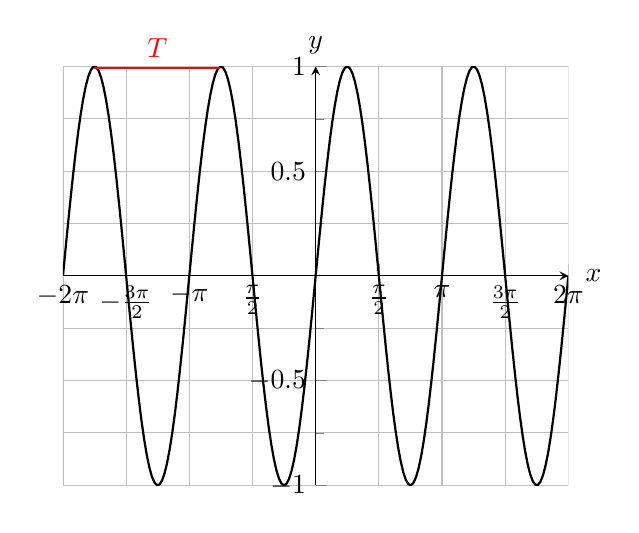
\begin{tikzpicture}
       	\pgfmathdeclarefunction{S}{2}{\pgfmathparse{sin(deg(#1*#2))}}
      	\begin{axis}[
    xtick={
        -6.28318, -4.7123889, -3.14159, -1.5708,
        1.5708, 3.14159, 4.7123889, 6.28318
    },
    xticklabels={
        $-2\pi$, $-\frac{3\pi}{2}$, $-\pi$, $\frac{\pi}{2}$,
        $\frac{\pi}{2}$, $\pi$, $\frac{3\pi}{2}$, $2\pi$
    },
    axis lines = center,
    grid=both,minor tick num=1,
    xlabel=$x$,ylabel=$y$,
    tick align=inside,
        legend style={at={(0.5,-0.1)},
        anchor=north,legend columns=2},
        domain=-2*pi:2*pi,
        samples=200,
        every axis y label/.style={rotate=0, black, at={(0.5,1.05)},},
        every axis x label/.style={rotate=0, black, at={(1.05,0.5)},},
        ]
        \addplot [thick] {S(2,x)};
       \end{axis}
        \draw[red,thick]  (0.4,5.3) to ["$T$"] (2,5.3);
	\end{tikzpicture}\\
\end{figure}
{La fréquence $F$ (en Hz) représente le nombre de répétitions de la perturbation par secondes.}\\
{On peut l'exprimer en fonction de la période $T$}
\[F=\frac{1}{T}\]

\subsection{Longueur d'onde}
{La longueur d'onde $\lambda$ est la distance pour qu'un point revienne dans un même état vibratoire}\\
{On peut lier la longueur d'onde, la célérité et la période d'une onde avec cette formule:}
\[c=\frac{\lambda}{T}\quad\Leftrightarrow\quad c=\lambda \times F\]

\section{Ondes sonores}
\subsection{Analyse spectrale}
{Un son est caractérisé par}
\begin{itemize}
  	\item{Sa hauteur, qui permet de dire s'il est grave ou aigu ou de la rattacher à une note de musique}
  	\item{Son timbre, qui dépend de la source qui l'émet}
 \end{itemize}


\begin{center}
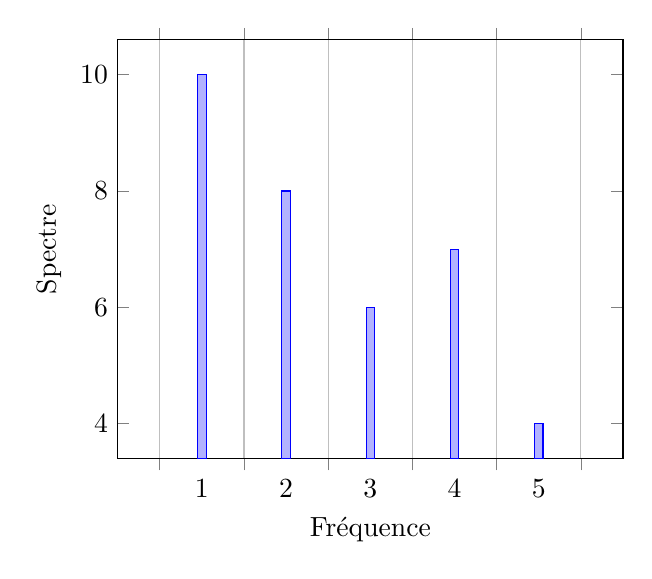
\begin{tikzpicture}
\begin{axis}[
	x tick label style={
		/pgf/number format/1000 sep=},
	ylabel=Spectre,
	xlabel=Fréquence,
	legend style={at={(0.5,-0.1)},
	anchor=north,legend columns=-1},
	ybar interval=0.1,
]
\addplot 
	coordinates {(1, 10) (2, 8)
		 (3,6) (4,7) (5,4) (6,7)};
\end{axis}
\end{tikzpicture}\\
\caption{Analyse spectrale d'un son}	
\end{center}

{La fréquence fondamentale est la plus petite et celle qui détermine la hauteur du son.}\\
{Les autres sont les harmoniques et déterminent le timbre du son.}\\

{Les fréquences des harmoniques sont multiples de la fréquence fondamentale donc}
\[F_n=F_0\times n\]

{Un son pur est composé d'une seule fréquence et un son complexe de plusieurs.}

\subsection{Intensité et niveau sonore}
{Le niveau sonore est défini par la relation suivante}
\[L=10\times \log \left(\frac{I}{I_0}\right)\]
{avec}
\begin{itemize}
  	\item{$L$ niveau sonore en $dB$}
  	\item{$I$ l'intensité acoustique de l'onde sonore en $W$.$m^{-2}$}
  	\item{$I_0$ le seuil d'audibilité fixé à $10^{-12}$ $W$.$m^{-2}$}
\end{itemize}

\section{Propriétés particulières des ondes}
\subsection{Effet Doppler}
{Si l'émetteur et le récepteur}
\begin{itemize}
  	\item{Se rapprochent, alors la fréquence augmente (et la longueur d'onde diminue)}
  	\item{S'éloignent, alors la fréquence diminue (et la longueur d'onde augmente)}
  	\item{Sont immobiles, alors la fréquence (et la longueur d'onde) reste la même}
\end{itemize}


\subsection{Diffraction}
{La diffraction est le phénomène d'éparpillement d'une onde (étalement des directions de propagation) à l'encontre d'un obstacle ou d'une ouverture}
\begin{center}
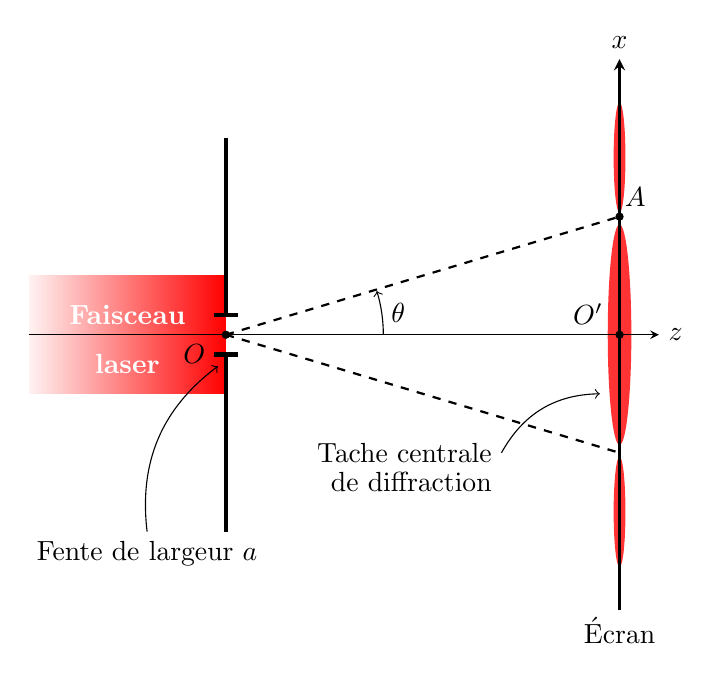
\begin{tikzpicture}[scale=0.5]
\shade[white, left color = red!05, right color = red] (-5,-1.5)rectangle(0,1.5) node[above, pos=0.5]{\textbf{Faisceau}};
\node[white] at (-2.5,-0.75) {\textbf{laser}};
\fill[red!80] (10,0) ellipse (0.3 and 2.8);
\fill[red!80] (10,4.5) ellipse (0.15 and 1.4);
\fill[red!80] (10,-4.5) ellipse (0.15 and 1.4);
\draw[->, >=stealth, thick] (10,-7)--(10,7) node[above]{$x$};
\node at (10,-7.5) {Écran};
\draw[->] (-2,-5)to[bend left](-0.2,-0.8) ;
\node[below] at (-2,-5) {Fente de largeur $a$};
\draw[->] (7,-3)to[bend left](9.5,-1.5) ;
\node[left] at (7,-3) {Tache centrale};
\node[left] at (7,-3.75) {de diffraction};
\draw[black, ultra thick] (0,-5)--(0,-0.5) ;
\draw[black, ultra thick] (0,0.5)--(0,5) ;
\draw[black, ultra thick] (-0.3,0.5)--(0.3,0.5) ;
\draw[black, ultra thick] (-0.3,-0.5)--(0.3,-0.5) ;
\draw[->] (4,0)arc(0:17:3.8) node[right, pos=0.5]{$\theta$};
\fill[black] (0,0)circle(3pt) node[left=0.4cm, below]{$O$};
\fill[black] (10,0)circle(3pt) node[left=0.4cm, above]{$O^{\prime}$};
\fill[black] (10,3)circle(3pt) node[right=0.2cm, above]{$A$};
\draw[dashed, thick] (0,0)--(10,3);
\draw[dashed, thick] (0,0)--(10,-3);
\draw[->, >=stealth] (-5,0)--(11,0) node[right]{$z$};
\end{tikzpicture}\\
\caption{Figure de diffraction}	
\end{center}

{L'écart angulaire $\theta$ est défini par}
\[\theta=\frac{\lambda}{a}\]

\subsection{Interférences}
{Le phénomène d'interférences se produit quand deux ondes monochromatiques de même nature et de même fréquence se superposent}


\begin{center}
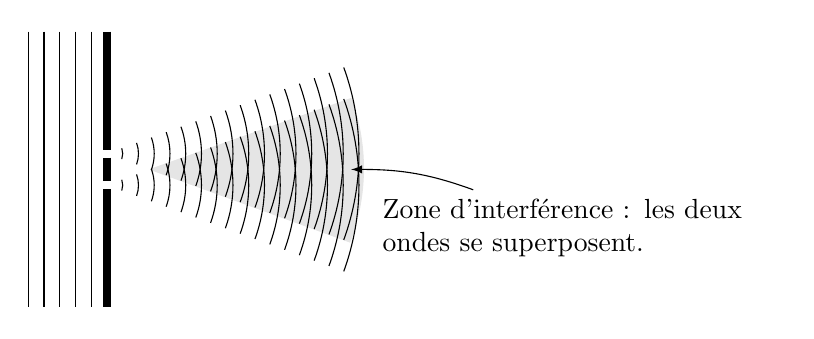
\begin{tikzpicture}[scale=0.05] 
\draw [line width=0.1cm] (0,70) -- (0,40); 
\draw [line width=0.1cm] (0,38) -- (0,32); 
\draw [line width=0.1cm] (0,30) -- (0,0); 
\foreach \x in {-4,-8,...,-20} \draw (\x,70) -- (\x,0) ; 
\filldraw [color=gray!20] (11,35) -- (62,53) arc (20:-21:52) -- (11,35); 
\foreach \x in {4,8,...,64} \draw ({\x*cos(20)},{39-\x*sin(20)}) arc (-20:20:\x) ; 
\foreach \x in {4,8,...,64} \draw ({\x*cos(20)},{31-\x*sin(20)}) arc (-20:20:\x); 
\node[text width=5cm] (I) at (120,20) {Zone d'interférence : les deux ondes se superposent.}; 
\draw[->,>=latex] (I) to[out=160,in=0] (62,35); 
\end{tikzpicture}\\
\caption{Figure de diffraction avec deux fentes}
\end{center}

{L'interfrange d'interférences $i$ est notée}
\[i=\frac{\lambda \times D}{e}\]

\end{document}